The {\em cosine circle} (also known as the second Lemoine circle) \cite[Cosine Circle]{mw} of a triangle passes through 6 points: the 3 pairs of intersections of sides with lines drawn through the symmedian $X_6$ parallel to sides of the orthic triangle. Recall that the orthic vertices are the feet of altitudes. Its center is $X_6$ \cite[Cosine Circle]{mw}. If one takes the excentral triangle of an orbit as the reference triangle, it is easy to see its orthic is the orbit itself; see Figure~\ref{sec:cosine-circle}.

\begin{theorem}
The cosine circle of the excentral triangle is invariant over the family of 3-periodic orbits. Its radius $r^*$ is constant and it is concentric and external to the elliptic billiard.
\label{thm:cosine-circle}
\end{theorem}

\begin{proof}
Once again, we set $P_1=(a,0)$, derive a candidate expression for $r^*$, and with a CAS check if the claim holds for all $x_1\in(-a,a)$. This yields

\begin{equation}
r^*=\frac{a^2-b^2}{\sqrt{2\delta-a^2-b^2}}\cdot
\end{equation}

Let $a>b>0$ and $\delta=\sqrt{a^4-a^2 b^2+b^4}$. As $0 < {(a^2-b^2)}^{2}<\delta^2$; it follows that
\begin{equation*} (r^{*})^{2}=  \frac{a^2+ b^2+2\delta}{3}
  > \; \frac{a^2+b^2+2(a^2-b^2)}{3} > \; a^2\cdot
\end{equation*}

As the excentral cosine circle and the elliptic billiard are concentric, the proof is complete.
\end{proof}

\begin{figure}[H]
    \centering
    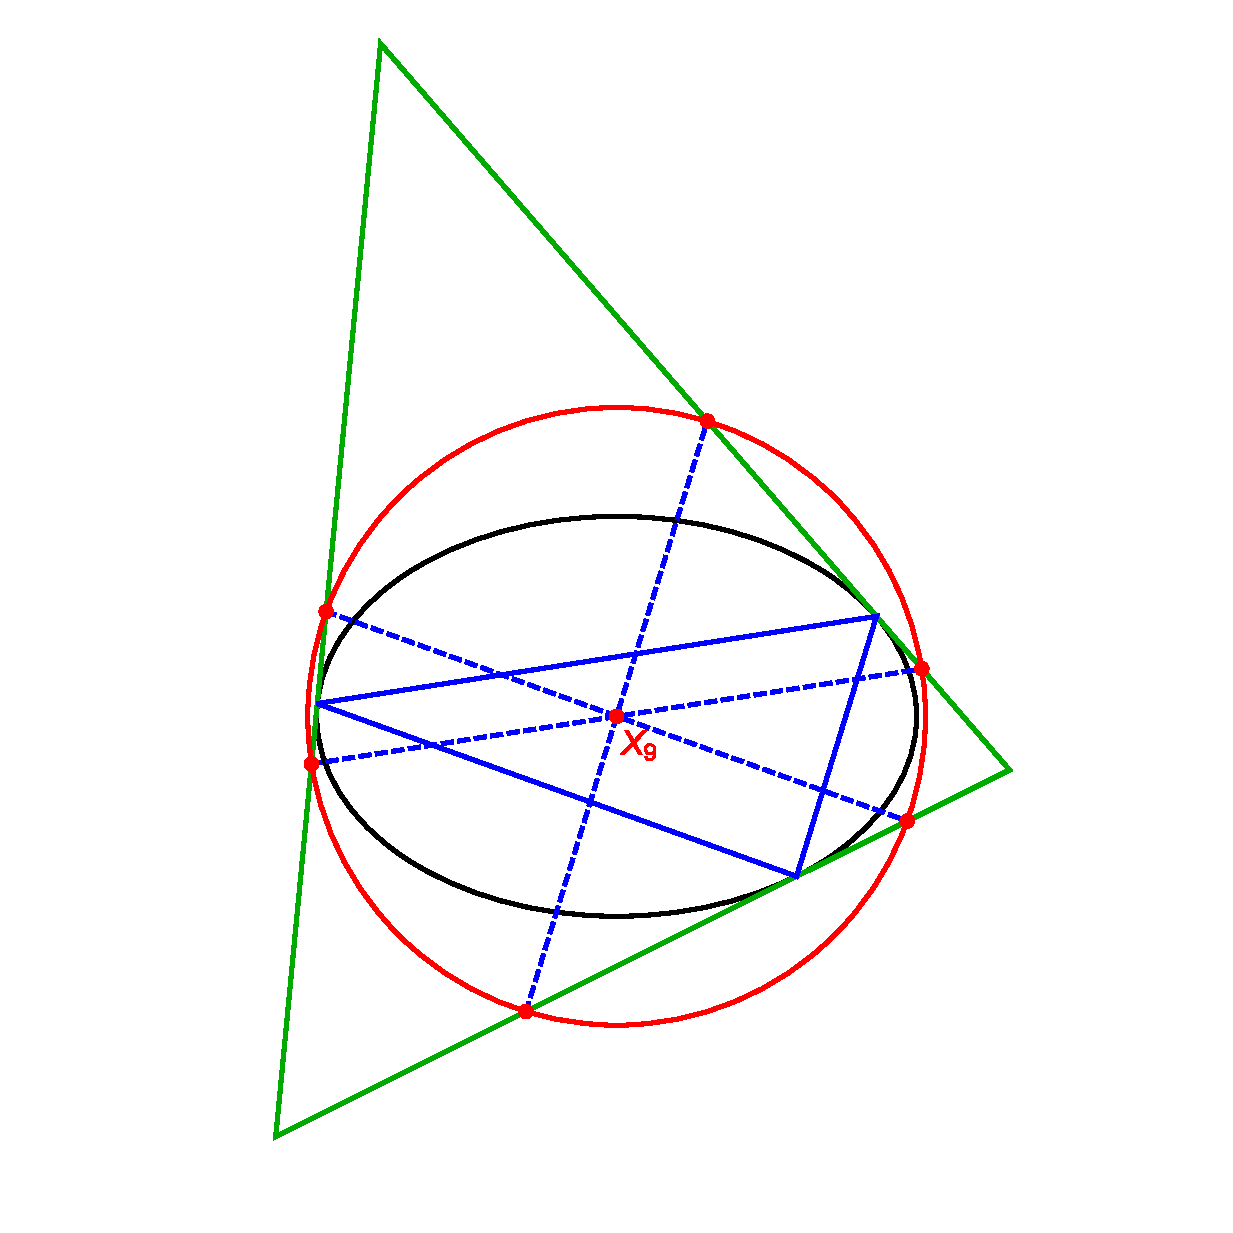
\includegraphics[width=.65\textwidth]{1080_cosine_circle_locus_antiparallels.eps}
    \caption{Given a 3-periodic orbit (blue), the cosine circle (red) of the excentral triangle (green) passes through the three pairs of intersections of the dashed lines with the excentral triangle. These are lines parallel to the orbit's sides drawn through the excentral's symmedian point $X_6$, congruent with the orbit's Mittenpunkt $X_9$. This circle is stationary across the 3-periodic orbit family and always exterior to the elliptic billiard. \textbf{Video:} \cite[PL\#04]{reznik2020-playlist-proofs}.}
    \label{fig:cos-circle}
\end{figure}

\begin{remark}
S. Tabachnikov kindly contributed 
\cite{reznik2019-intelligencer} the following equivalent expression for $r^*$, valid for all $N$:

\begin{equation}
    r^* = 1/\gamma\cdot
\label{eqn:rstar-sergei}
\end{equation}
\end{remark}

\begin{remark}[Youtube Math]

In the comments section to our cosine circle video \cite[PL\#05]{reznik2020-playlist-proofs}, D. Laurain contributed an alternative expression for $r^*$ \cite{dominique19}:

\begin{equation}
    r^* = \frac{2 L}{r/R+4}\cdot
    \label{eqn:rstar-laurain}
\end{equation}
\end{remark}

\noindent Combining this with $r^*=1/\gamma$ \eqref{eqn:rstar-sergei}, we obtain the following.

\begin{theorem}
${r/R}={\gamma}L-4$, where $\gamma$ is Joachimsthal's constant and $L$ is the orbit's perimeter.
\label{thm:rovR-explicit}
\end{theorem}